\section{Restliche Werte eingeben/�bersicht}Hier sehen Sie die �bersicht �ber alle zu erstellenden Clients. Nun k�nnen Sie die L�cken in den Tabellen f�llen bzw. Werte �ndern und �berpr�fen, ob die vorhandenen Werte Ihren Vorstellungen entsprechen.\\
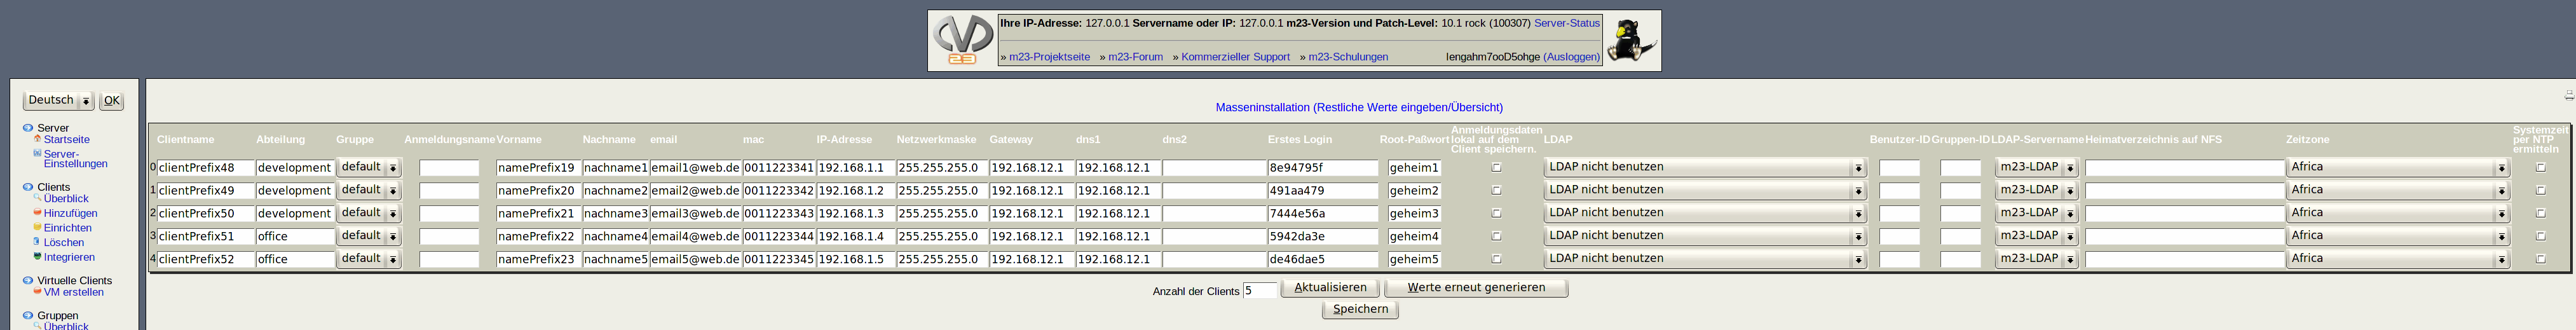
\includegraphics[scale=0.33]{/mdk/doc/manual/screenshots/de/mi_step4.png} \\
\subsection{Anzahl der Clients �ndern}
Sie k�nnen die Anzahl der Clients �ndern, indem Sie bei \textit{"Anzahl der Clients"} die neue Anzahl angeben und danach auf \textit{"Aktualisieren"} klicken, wenn Sie weniger Clients oder auf \textit{"Werte erneut generieren"}, wenn Sie mehr Clients als vorher w�nschen.\\
Werden mehr Clients als zuvor angegeben, so hat dies zur Folge, da� mit einem Klick auf "Werte erneut generieren" die Generatoren die ben�tigten Werte erstellen, bzw. zus�tzliche Werte aus der Datenbank-Datei gelesen werden. Sollten aus der Datenbank-Datei nicht gen�gend Werte ausgelesen werden k�nnen, so m�ssen dieser per Hand in die Tabelle eingegeben werden. Die Generierung von vielen Werten kann u.U. sehr lange dauern, z.B. wenn die IP-Adressen generiert werden sollen und Sie ausgew�hlt haben, da� die IP-Adressen vor Benutzung "angepingt" werden sollen.\\
Klicken Sie abschlie�end auf \textit{"Speichern"}, um die Installation auf den Clients zu starten.\\
